%!TeX root=../emmatop.tex
\chapter[Chapter \thechapter]{}
\lettrine[lraise=0.3]{T}{he} very day of Mr Elton's going to London produced a fresh occasion for Emma's services towards her friend. Harriet had been at Hartfield, as usual, soon after breakfast; and, after a time, had gone home to return again to dinner: she returned, and sooner than had been talked of, and with an agitated, hurried look, announcing something extraordinary to have happened which she was longing to tell. Half a minute brought it all out. She had heard, as soon as she got back to Mrs Goddard's, that Mr Martin had been there an hour before, and finding she was not at home, nor particularly expected, had left a little parcel for her from one of his sisters, and gone away; and on opening this parcel, she had actually found, besides the two songs which she had lent Elizabeth to copy, a letter to herself; and this letter was from him, from Mr Martin, and contained a direct proposal of marriage. <Who could have thought it? She was so surprized she did not know what to do. Yes, quite a proposal of marriage; and a very good letter, at least she thought so. And he wrote as if he really loved her very much—but she did not know—and so, she was come as fast as she could to ask Miss Woodhouse what she should do.\longdash> Emma was half-ashamed of her friend for seeming so pleased and so doubtful.

<Upon my word,> she cried, <the young man is determined not to lose any thing for want of asking. He will connect himself well if he can.>

<Will you read the letter?> cried Harriet. <Pray do. II'd rather you would.>

Emma was not sorry to be pressed. She read, and was surprized. The style of the letter was much above her expectation. There were not merely no grammatical errors, but as a composition it would not have disgraced a gentleman; the language, though plain, was strong and unaffected, and the sentiments it conveyed very much to the credit of the writer. It was short, but expressed good sense, warm attachment, liberality, propriety, even delicacy of feeling. She paused over it, while Harriet stood anxiously watching for her opinion, with a <Well, well,> and was at last forced to add, <Is it a good letter? or is it too short?>

<Yes, indeed, a very good letter,> replied Emma rather slowly—<so good a letter, Harriet, that every thing considered, I think one of his sisters must have helped him. I can hardly imagine the young man whom I saw talking with you the other day could express himself so well, if left quite to his own powers, and yet it is not the style of a woman; no, certainly, it is too strong and concise; not diffuse enough for a woman. No doubt he is a sensible man, and I suppose may have a natural talent for—thinks strongly and clearly—and when he takes a pen in hand, his thoughts naturally find proper words. It is so with some men. Yes, I understand the sort of mind. Vigorous, decided, with sentiments to a certain point, not coarse. A better written letter, Harriet (returning it,) than I had expected.>

<Well,> said the still waiting Harriet;—<well—and—and what shall I do?>

<What shall you do! In what respect? Do you mean with regard to this letter?>

<Yes.>

<But what are you in doubt of? You must answer it of course—and speedily.>

<Yes. But what shall I say? Dear Miss Woodhouse, do advise me.>

<Oh no, no! the letter had much better be all your own. You will express yourself very properly, I am sure. There is no danger of your not being intelligible, which is the first thing. Your meaning must be unequivocal; no doubts or demurs: and such expressions of gratitude and concern for the pain you are inflicting as propriety requires, will present themselves unbidden to \textit{your} mind, I am persuaded. You need not be prompted to write with the appearance of sorrow for his disappointment.>

<You think I ought to refuse him then,> said Harriet, looking down.

<Ought to refuse him! My dear Harriet, what do you mean? Are you in any doubt as to that? I thought—but I beg your pardon, perhaps I have been under a mistake. I certainly have been misunderstanding you, if you feel in doubt as to the \textit{purport} of your answer. I had imagined you were consulting me only as to the wording of it.>

Harriet was silent. With a little reserve of manner, Emma continued:

<You mean to return a favourable answer, I collect.>

<No, I do not; that is, I do not mean—What shall I do? What would you advise me to do? Pray, dear Miss Woodhouse, tell me what I ought to do.>

<I shall not give you any advice, Harriet. I will have nothing to do with it. This is a point which you must settle with your feelings.>

<I had no notion that he liked me so very much,> said Harriet, contemplating the letter. For a little while Emma persevered in her silence; but beginning to apprehend the bewitching flattery of that letter might be too powerful, she thought it best to say,

<I lay it down as a general rule, Harriet, that if a woman \textit{doubts} as to whether she should accept a man or not, she certainly ought to refuse him. If she can hesitate as to <Yes,> she ought to say <No> directly. It is not a state to be safely entered into with doubtful feelings, with half a heart. I thought it my duty as a friend, and older than yourself, to say thus much to you. But do not imagine that I want to influence you.>

<Oh! no, I am sure you are a great deal too kind to—but if you would just advise me what I had best do—No, no, I do not mean that—As you say, one's mind ought to be quite made up—One should not be hesitating—It is a very serious thing.—It will be safer to say <No,> perhaps.—Do you think I had better say <No>?>

<Not for the world,> said Emma, smiling graciously, <would I advise you either way. You must be the best judge of your own happiness. If you prefer Mr Martin to every other person; if you think him the most agreeable man you have ever been in company with, why should you hesitate? You blush, Harriet.—Does any body else occur to you at this moment under such a definition? Harriet, Harriet, do not deceive yourself; do not be run away with by gratitude and compassion. At this moment whom are you thinking of?>

The symptoms were favourable.—Instead of answering, Harriet turned away confused, and stood thoughtfully by the fire; and though the letter was still in her hand, it was now mechanically twisted about without regard. Emma waited the result with impatience, but not without strong hopes. At last, with some hesitation, Harriet said—

<Miss Woodhouse, as you will not give me your opinion, I must do as well as I can by myself; and I have now quite determined, and really almost made up my mind—to refuse Mr Martin. Do you think I am right?>

<Perfectly, perfectly right, my dearest Harriet; you are doing just what you ought. While you were at all in suspense I kept my feelings to myself, but now that you are so completely decided I have no hesitation in approving. Dear Harriet, I give myself joy of this. It would have grieved me to lose your acquaintance, which must have been the consequence of your marrying Mr Martin. While you were in the smallest degree wavering, I said nothing about it, because I would not influence; but it would have been the loss of a friend to me. I could not have visited Mrs Robert Martin, of Abbey-Mill Farm. Now I am secure of you for ever.>

Harriet had not surmised her own danger, but the idea of it struck her forcibly.

<You could not have visited me!> she cried, looking aghast. <No, to be sure you could not; but I never thought of that before. That would have been too dreadful!—What an escape!—Dear Miss Woodhouse, I would not give up the pleasure and honour of being intimate with you for any thing in the world.>

<Indeed, Harriet, it would have been a severe pang to lose you; but it must have been. You would have thrown yourself out of all good society. I must have given you up.>

<Dear me!—How should I ever have borne it! It would have killed me never to come to Hartfield any more!>

<Dear affectionate creature!—\textit{You} banished to Abbey-Mill Farm!—\textit{You} confined to the society of the illiterate and vulgar all your life! I wonder how the young man could have the assurance to ask it. He must have a pretty good opinion of himself.>

<I do not think he is conceited either, in general,> said Harriet, her conscience opposing such censure; <at least, he is very good natured, and I shall always feel much obliged to him, and have a great regard for—but that is quite a different thing from—and you know, though he may like me, it does not follow that I should—and certainly I must confess that since my visiting here I have seen people—and if one comes to compare them, person and manners, there is no comparison at all, \textit{one} is so very handsome and agreeable. However, I do really think Mr Martin a very amiable young man, and have a great opinion of him; and his being so much attached to me—and his writing such a letter—but as to leaving you, it is what I would not do upon any consideration.>

<Thank you, thank you, my own sweet little friend. We will not be parted. A woman is not to marry a man merely because she is asked, or because he is attached to her, and can write a tolerable letter.>

<Oh no;—and it is but a short letter too.>

Emma felt the bad taste of her friend, but let it pass with a <very true; and it would be a small consolation to her, for the clownish manner which might be offending her every hour of the day, to know that her husband could write a good letter.>

<Oh! yes, very. Nobody cares for a letter; the thing is, to be always happy with pleasant companions. I am quite determined to refuse him. But how shall I do? What shall I say?>

Emma assured her there would be no difficulty in the answer, and advised its being written directly, which was agreed to, in the hope of her assistance; and though Emma continued to protest against any assistance being wanted, it was in fact given in the formation of every sentence. The looking over his letter again, in replying to it, had such a softening tendency, that it was particularly necessary to brace her up with a few decisive expressions; and she was so very much concerned at the idea of making him unhappy, and thought so much of what his mother and sisters would think and say, and was so anxious that they should not fancy her ungrateful, that Emma believed if the young man had come in her way at that moment, he would have been accepted after all.

This letter, however, was written, and sealed, and sent. The business was finished, and Harriet safe. She was rather low all the evening, but Emma could allow for her amiable regrets, and sometimes relieved them by speaking of her own affection, sometimes by bringing forward the idea of Mr Elton.

<I shall never be invited to Abbey-Mill again,> was said in rather a sorrowful tone.

<Nor, if you were, could I ever bear to part with you, my Harriet. You are a great deal too necessary at Hartfield to be spared to Abbey-Mill.>

<And I am sure I should never want to go there; for I am never happy but at Hartfield.>

Some time afterwards it was, <I think Mrs Goddard would be very much surprized if she knew what had happened. I am sure Miss Nash would—for Miss Nash thinks her own sister very well married, and it is only a linen-draper.>

<One should be sorry to see greater pride or refinement in the teacher of a school, Harriet. I dare say Miss Nash would envy you such an opportunity as this of being married. Even this conquest would appear valuable in her eyes. As to any thing superior for you, I suppose she is quite in the dark. The attentions of a certain person can hardly be among the tittle-tattle of Highbury yet. Hitherto I fancy you and I are the only people to whom his looks and manners have explained themselves.>

Harriet blushed and smiled, and said something about wondering that people should like her so much. The idea of Mr Elton was certainly cheering; but still, after a time, she was tender-hearted again towards the rejected Mr Martin.

<Now he has got my letter,> said she softly. <I wonder what they are all doing—whether his sisters know—if he is unhappy, they will be unhappy too. I hope he will not mind it so very much.>

\begin{figure}[tbph]
\centering
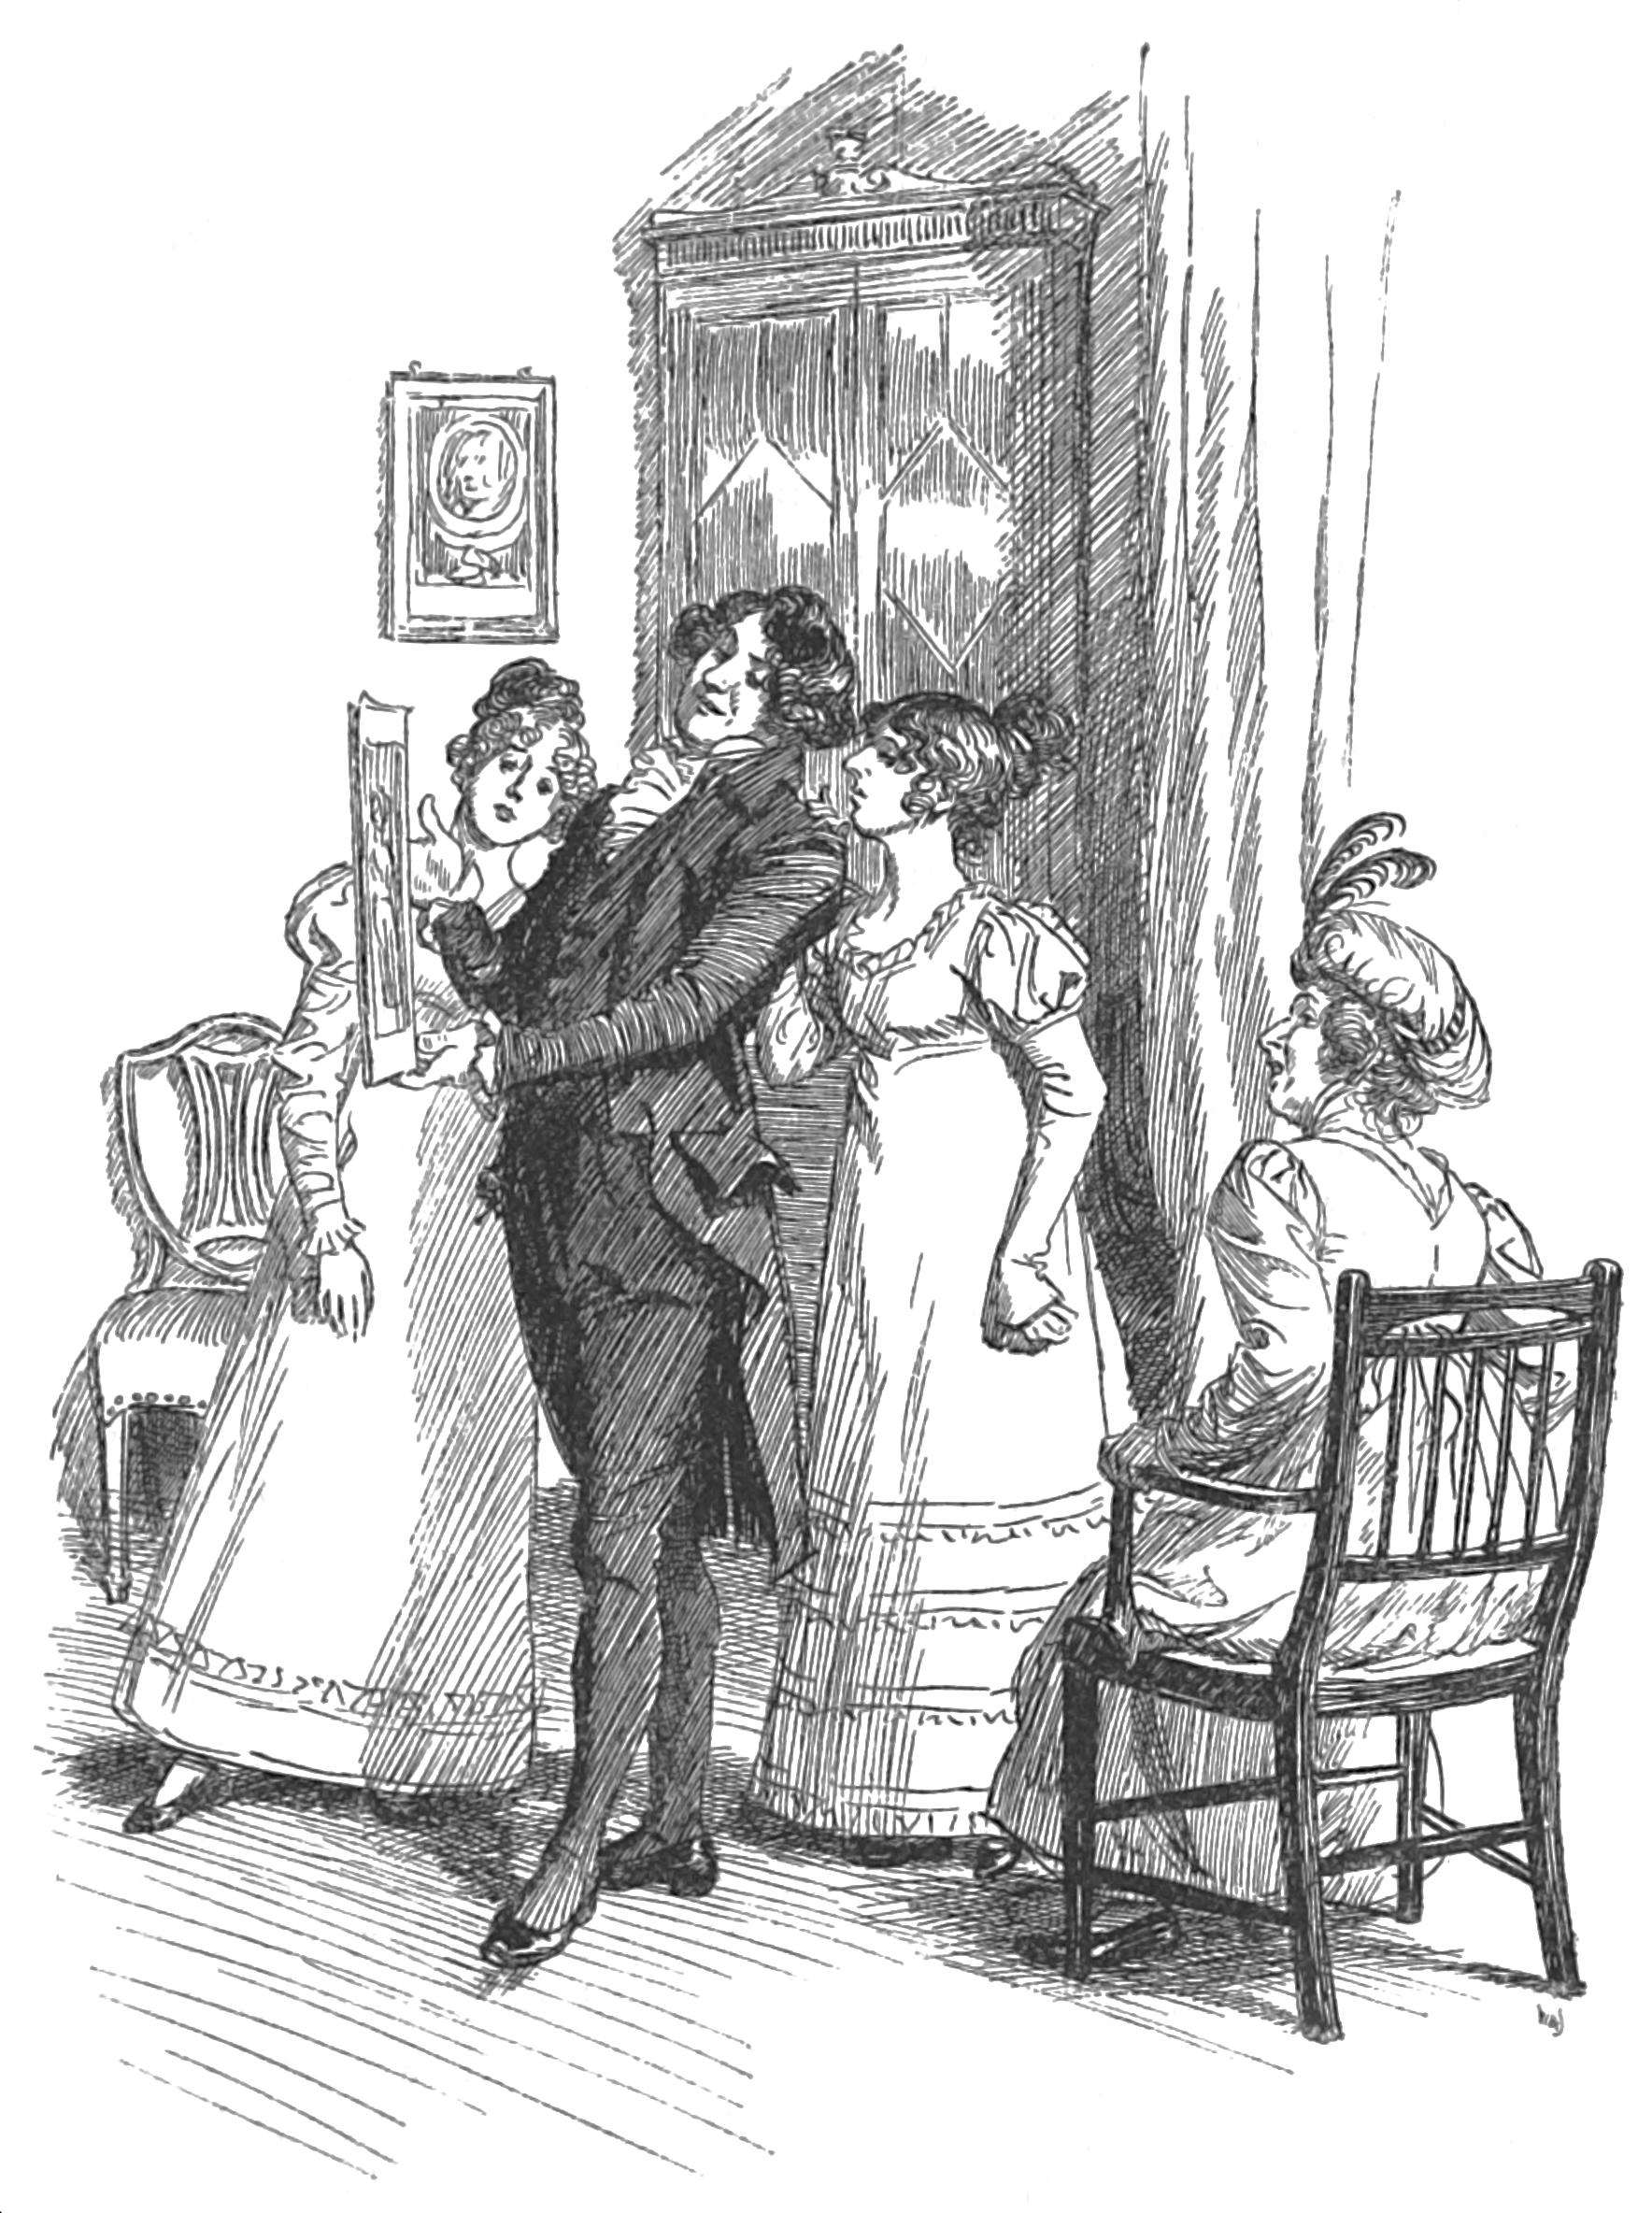
\includegraphics[width=.9\linewidth]{7portrait}
\caption{<Shewing your picture to his mother and sisters>}
\end{figure}

<Let us think of those among our absent friends who are more cheerfully employed,> cried Emma. <At this moment, perhaps, Mr Elton is shewing your picture to his mother and sisters, telling how much more beautiful is the original, and after being asked for it five or six times, allowing them to hear your name, your own dear name.>

<My picture!—But he has left my picture in Bond-street.>

<Has he so!—Then I know nothing of Mr Elton. No, my dear little modest Harriet, depend upon it the picture will not be in Bond-street till just before he mounts his horse to-morrow. It is his companion all this evening, his solace, his delight. It opens his designs to his family, it introduces you among them, it diffuses through the party those pleasantest feelings of our nature, eager curiosity and warm prepossession. How cheerful, how animated, how suspicious, how busy their imaginations all are!>

Harriet smiled again, and her smiles grew stronger.